\section{EException Class Reference}
\label{classEException}\index{EException@{EException}}
{\tt \#include $<$exception.hpp$>$}

Inheritance diagram for EException::\begin{figure}[H]
\begin{center}
\leavevmode
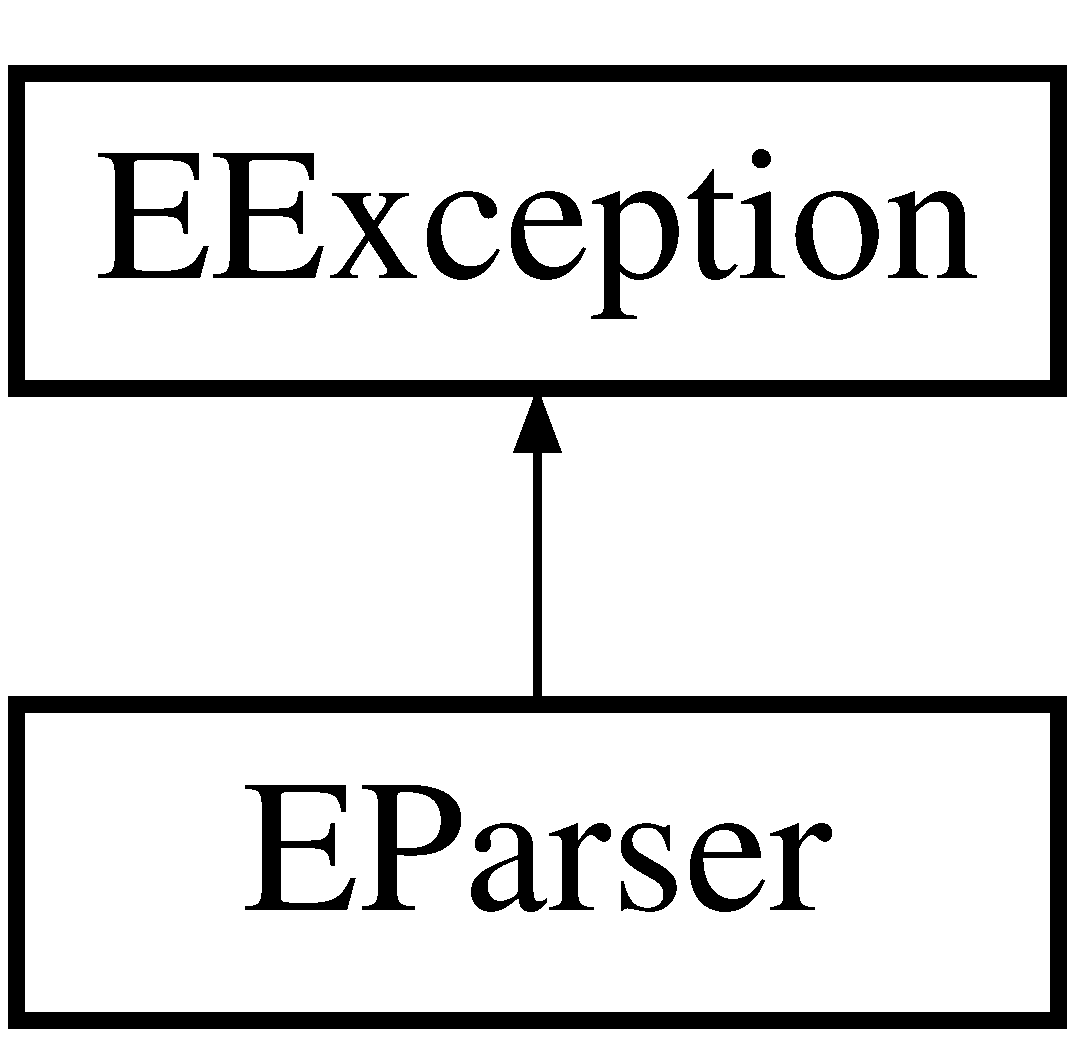
\includegraphics[height=2cm]{classEException}
\end{center}
\end{figure}
\subsection*{Public Member Functions}
\begin{CompactItemize}
\item 
{\bf EException} (QString message)
\item 
virtual {\bf $\sim$EException} ()
\item 
virtual QString {\bf message} ()
\end{CompactItemize}
\subsection*{Protected Attributes}
\begin{CompactItemize}
\item 
QString {\bf \_\-message}
\end{CompactItemize}


\subsection{Constructor \& Destructor Documentation}
\index{EException@{EException}!EException@{EException}}
\index{EException@{EException}!EException@{EException}}
\subsubsection{\setlength{\rightskip}{0pt plus 5cm}{\bf EException} (QString {\em message})\hspace{0.3cm}{\tt  [inline]}}\label{classEException_a0}


\index{EException@{EException}!~EException@{$\sim$EException}}
\index{~EException@{$\sim$EException}!EException@{EException}}
\subsubsection{\setlength{\rightskip}{0pt plus 5cm}virtual $\sim${\bf EException} ()\hspace{0.3cm}{\tt  [inline, virtual]}}\label{classEException_a1}




\subsection{Member Function Documentation}
\index{EException@{EException}!message@{message}}
\index{message@{message}!EException@{EException}}
\subsubsection{\setlength{\rightskip}{0pt plus 5cm}virtual QString message ()\hspace{0.3cm}{\tt  [inline, virtual]}}\label{classEException_a2}




\subsection{Member Data Documentation}
\index{EException@{EException}!_message@{\_\-message}}
\index{_message@{\_\-message}!EException@{EException}}
\subsubsection{\setlength{\rightskip}{0pt plus 5cm}QString {\bf \_\-message}\hspace{0.3cm}{\tt  [protected]}}\label{classEException_p0}




The documentation for this class was generated from the following file:\begin{CompactItemize}
\item 
{\bf exception.hpp}\end{CompactItemize}
